\section{Official Protocols: Reproduction, Comparison and What the Scores Are Made Of}
\label{sec:official}

\subsection{Reproducing BladeYOLO, and Why Our Results Differed}
\label{sec:history}
We report this history in full because the same traps face anyone who works on these datasets. Fig.~\ref{fig:history} gives the sequence, and Table~\ref{tab:runs} the original runs on the Wind Surface split used by BladeYOLO (2{,}856 train/714 validation).

\textbf{Phase 1: a faithful reimplementation.} From the paper we rebuilt frozen DINOv3 ViT-S/16 tapped at blocks 4/8/12, Fourier-amplitude style injection into those blocks, a WTConv detail branch~\cite{wtconv}, Cross-Mamba P5$\rightarrow$P4$\rightarrow$P3 guidance and the YOLOv12-L neck and head~\cite{bladeyolo}. The first two runs failed: Run 1 hit bf16, unfreezing and distributed-training failures, and Run 2 produced NaNs from FFT gradients. Run 3, with the FFT detached and SGD, stagnated at about 52.6/28.0, which is 33.9/29.4 points below the published 86.5/57.4. That gap is far beyond run-to-run variance.

\textbf{Phase 2: our own variants.} A small model without style injection or Mamba (BladeYOLO-S, 8\,M parameters) reached 64.3/37.3. A large one with deformable ``morphological'' convolutions and learnable wavelets (BladeYOLO-L, 57.2\,M, AdamW) then reached 78.2/46.9. Adding a ``Cross-Scale Vision Mamba'' and WIoU v3 gave 77.0/47.8, and we credited WIoU with $+0.9$ \mcoco.

\textbf{Phase 3: the code audit.} An audit of all model code showed that Run 7 was not the model we had described. The WIoU patch reached the wrong namespace, so Run 7 trained with plain CIoU; the formula also had three errors. The ``Mamba'' block did not perform a selective scan. The DINOv3 extractor skipped RoPE and fed unnormalised pixels, so every run before 9 October used weakened features. And the wavelet branch threw away high-frequency detail. All four were repaired and unit-tested (Section~\ref{sec:byv2}).

\textbf{Phase 4: the leak.} A pixel comparison then showed that 75\% (later 84\%) of the Wind Surface validation images had a training twin. Of the 1{,}785 augmented \texttt{\_0}/\texttt{\_1} pairs, 550 are split across train and validation. We merged Wind Surface and WTBlade-Defect into a deduplicated, group-split dataset (v2: 2{,}606 unique images out of 11{,}681). On it, stock YOLO12-L scored 35.8/14.9 and the repaired BladeYOLO-L 40.0/14.6. A larger, taxonomy-mapped v3 (5{,}777 images from five sources) scored only 26--32 \mfifty. Its classes rest on few independent scenes, and one class had a single training group. An exhaustive review of 763 label candidates on v3 was worth only $+3$ \mfifty, and a three-model weighted-box-fusion ensemble~\cite{wbf} about $+3$ when its fusion IoU was chosen on validation. Only then did the audit lead us to WTBD alone, with its native classes, and to the leak-free benchmarks of Section~\ref{sec:benchmarks}.

\textbf{Why our reproduction differs from the paper.} Four causes are documented. (i) The paper reports 3{,}790 Wind Surface images, while the public copy has 3{,}570. (ii) No split seed, image list or code is published, and the WTBlade numbers use an unpublished 9:1 re-split. (iii) Our early runs had the code defects above, so they support ``not reproducible from the published information'' and not ``the published modules do not work''. (iv) Any random split of these data is dominated by twins (Section~\ref{sec:audit}). That last cause also makes a high number easy to obtain and impossible to interpret. Note that our 78.2/46.9 was itself a leaked number.

\begin{figure}[!t]
\centering
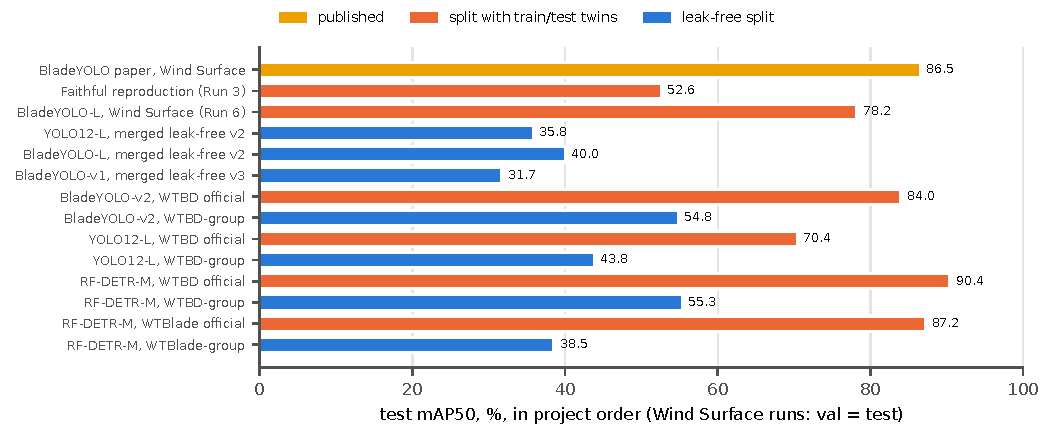
\includegraphics[width=\linewidth]{fig23_score_history}
\caption{Reported \mfifty at each stage of the project, in order. Every class-aware score above about 60 was measured on a split with train/test twins, including our own. Datasets differ between rows, so rows are not comparable as models; the point is the pattern.}
\label{fig:history}
\end{figure}

\begin{table}[!t]
\centering
\caption{Early runs on the original Wind Surface split (2{,}856/714), \mfifty/\mcoco on validation. Later analysis invalidated the conclusions drawn from them.}
\label{tab:runs}
\footnotesize
\begin{tabularx}{\linewidth}{@{}l X r r X@{}}
\toprule
Run & Architecture & \mfifty & \mcoco & Outcome \\
\midrule
1--2 & Faithful: DINOv3 + style injection + WTConv + Cross-Mamba & -- & -- & bf16, unfreezing, DDP failures; FFT NaNs \\
3 & Faithful, FFT detached, SGD, $\sim$283 ep & $\sim$52.6 & $\sim$28.0 & stagnated; closest reproduction \\
4 & BladeYOLO-S (8\,M), 400 ep & 64.3 & 37.3 & apparent ceiling \\
6 & BladeYOLO-L (57.2\,M), AdamW, 400 ep & 78.2 & 46.9 & ``breakthrough'' (leaked) \\
7 & Run 6 + ``Mamba'' + WIoU v3 & 77.0 & 47.8 & WIoU never ran; no scan \\
\bottomrule
\end{tabularx}
\end{table}

\subsection{Our Numbers Against Published Ones}
Table~\ref{tab:cross} brings every model we trained or reproduced together with the published results, across the three official and the two leak-free benchmarks. Read by column, it shows three things. No single model leads everywhere. The official columns are 25--50 points higher than the leak-free ones for the same model. And the published BladeYOLO numbers stand alone on the two protocols on which they were reported.

\begin{table*}[!t]
\centering
\caption{Comparison across all five benchmarks: \mfifty / \mcoco on the test set of each protocol (Wind Surface: its validation set, which serves as test). Official protocols are leaky (Table~\ref{tab:audit}); leak-free ones are scene-grouped (Section~\ref{sec:benchmarks}). Two-seed means where two seeds exist. Our values use the COCO-style evaluator. \hlnote{} Shaded: proposed method.}
\label{tab:cross}
\footnotesize
\setlength{\tabcolsep}{3.4pt}
\begin{tabular}{@{}l c cc cc cc cc cc@{}}
\toprule
& & \multicolumn{6}{c}{\textit{Official protocols (leaky)}} & \multicolumn{4}{c}{\textit{Leak-free protocols (ours)}} \\
\cmidrule(lr){3-8}\cmidrule(l){9-12}
& & \multicolumn{2}{c}{WTBD-official} & \multicolumn{2}{c}{Wind Surface} & \multicolumn{2}{c}{WTBlade-Defect} & \multicolumn{2}{c}{WTBD-group} & \multicolumn{2}{c}{WTBlade-group} \\
\cmidrule(lr){3-4}\cmidrule(lr){5-6}\cmidrule(lr){7-8}\cmidrule(lr){9-10}\cmidrule(l){11-12}
Model & Source & 50 & 50:95 & 50 & 50:95 & 50 & 50:95 & 50 & 50:95 & 50 & 50:95 \\
\midrule
\multicolumn{12}{@{}l}{\textit{Published}} \\
BladeYOLO~\cite{bladeyolo} & paper & -- & -- & \best{86.5} & \best{57.4} & \second{85.8}$^\ddagger$ & \best{74.6}$^\ddagger$ & -- & -- & -- & -- \\
YOLOv12-L, as reported in~\cite{bladeyolo} & paper & -- & -- & -- & -- & 83.3$^\ddagger$ & \second{71.9}$^\ddagger$ & -- & -- & -- & -- \\
\midrule
\multicolumn{12}{@{}l}{\textit{Our reproductions of BladeYOLO (before the code audit and the leak finding)}} \\
Faithful reimplementation (Run 3) & ours & -- & -- & 52.6 & 28.0 & -- & -- & -- & -- & -- & -- \\
BladeYOLO-L (Run 6) & ours & -- & -- & 78.2 & 46.9 & -- & -- & -- & -- & -- & -- \\
\midrule
\multicolumn{12}{@{}l}{\textit{YOLO family}} \\
YOLO12-L~\cite{yolov12} & ours & 69.0 & 37.7 & -- & -- & -- & -- & 40.0 & 18.5 & 32.2 & 13.3 \\
BladeYOLO-v2 without DINOv3 & ours & -- & -- & -- & -- & -- & -- & 31.8 & 15.2 & -- & -- \\
BladeYOLO-v2 (frozen DINOv3)$^\S$ & ours & 81.5 & 48.1 & -- & -- & -- & -- & \second{56.1} & 24.4 & \best{41.8} & \best{18.0} \\
\midrule
\multicolumn{12}{@{}l}{\textit{Detection transformers}} \\
RF-DETR-L~\cite{rfdetr} (G26) & ours & 88.9 & 59.5 & -- & -- & -- & -- & -- & -- & -- & -- \\
RF-DETR-M~\cite{rfdetr} (G26 / A0) & ours & \second{90.4} & \best{61.2} & 81.0 & \second{53.3} & \best{87.2} & 55.1 & 54.3 & \second{32.2} & 40.0 & 16.6 \\
RF-DETR-M + copy-paste (G27 A1) & ours & -- & -- & -- & -- & -- & -- & 55.0 & 31.7 & 40.6 & 16.9 \\
\ours RF-DETR-FP (G29) & ours & \best{90.9} & \second{59.9} & \second{82.1} & 51.7 & -- & -- & \best{58.9} & \best{34.4} & \second{41.0} & \second{17.3} \\
\bottomrule
\end{tabular}
\tabnote{$^\ddagger$On BladeYOLO's own unpublished 9:1 re-split of 5{,}326 WTBlade-Defect images, not the official 553-image test set. Wind Surface: the BladeYOLO paper reports 3{,}790 images, our public copy has 3{,}570. $^\S$ViT-S/16 on WTBD, ViT-B/16 on WTBlade-group. Run 3 and Run 6 were measured with weakened DINOv3 features and other code defects (Section~\ref{sec:history}). RF-DETR-FP on WTBlade-Defect official was not run (pre-registered: it does not fit a 12\,h T4 session).}
\end{table*}

Table~\ref{tab:official} and Fig.~\ref{fig:official-bladeyolo} give our scores on the official protocols beside the published ones. A generic detector with a standard recipe and no blade-specific modules reaches the level of the specialised models on two protocols, but not on Wind Surface.

\begin{table}[!t]
\centering
\caption{Official protocols in detail: this work against published results. \mfifty/\mcoco [95\% CI], single seed, selected on validation; intervals are image-level. BladeYOLO's WTBlade numbers use its own unpublished 9:1 re-split, so that row is not directly comparable. $^\dagger$Ultralytics \texttt{val}; other rows of ours use the COCO-style evaluator. \hlnote{} (within each protocol)}
\label{tab:official}
\footnotesize
\setlength{\tabcolsep}{3pt}
\begin{tabularx}{\linewidth}{@{}X l@{}}
\toprule
Model & \mfifty / \mcoco \\
\midrule
\multicolumn{2}{@{}l}{\textit{WTBD-official (test 161)}} \\
YOLO12-L (ours)$^\dagger$ & 70.4 / 38.8 \\
BladeYOLO-v2 (ours)$^\dagger$ & 84.0 / 49.3 \\
RF-DETR-M 768, constant LR (G25) & \second{90.5} \ci{86.3}{94.4} / \second{60.2} \ci{55.6}{65.3} \\
RF-DETR-M 768, cosine (G26) & 90.4 \ci{85.8}{94.7} / \best{61.2} \ci{56.5}{66.1} \\
RF-DETR-L 704, cosine (G26) & 88.9 / 59.5 \\
\ours RF-DETR-FP 768 (G29) & \best{90.9} \ci{87.0}{94.6} / 59.9 \ci{55.2}{65.5} \\
\midrule
\multicolumn{2}{@{}l}{\textit{Wind Surface (val 714)}} \\
BladeYOLO~\cite{bladeyolo} & \best{86.5} / \best{57.4} \\
Faithful reimplementation (Run 3) & 52.6 / 28.0 \\
Our best leaky BladeYOLO-L (Run 6) & 78.2 / 46.9 \\
RF-DETR-M 640, 60 ep, constant (G25) & 81.8 \ci{78.0}{85.4} / 51.4 \ci{48.3}{55.0} \\
RF-DETR-M 640, 100 ep, cosine (G26) & 81.0 \ci{77.1}{84.9} / \second{53.3} \ci{50.0}{57.0} \\
\ours RF-DETR-FP 640, 100 ep (G29) & \second{82.1} \ci{78.4}{86.0} / 51.7 \ci{48.5}{55.4} \\
\midrule
\multicolumn{2}{@{}l}{\textit{WTBlade-Defect (test 553)}} \\
BladeYOLO~\cite{bladeyolo} & 85.8 / \best{74.6} \\
YOLOv12-L, as reported there & 83.3 / \second{71.9} \\
RF-DETR-M 640, 25 ep, constant (G25) & \best{87.4} \ci{84.4}{90.9} / 52.5 \ci{49.6}{56.2} \\
RF-DETR-M 640, 40 ep, cosine (G26) & \second{87.2} \ci{84.0}{90.6} / 55.1 \ci{52.0}{59.1} \\
\bottomrule
\end{tabularx}
\end{table}

\begin{figure*}[!t]
\centering
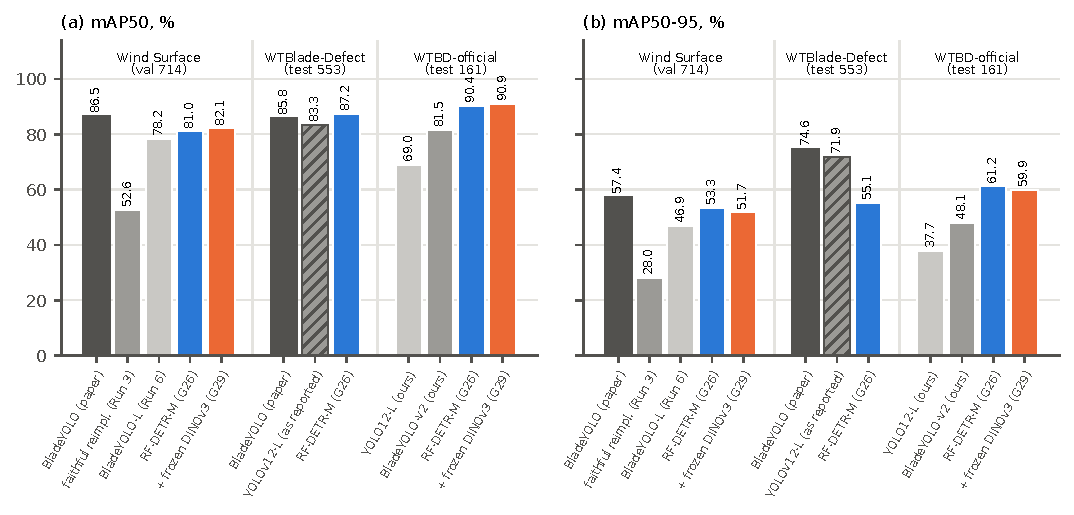
\includegraphics[width=0.92\textwidth]{fig32_official_vs_bladeyolo}
\caption{Official protocols: the BladeYOLO paper (dark), values reported in that paper for its baseline (hatched), our reproductions and BladeYOLO-style models (grey), RF-DETR-M with the G26 recipe (blue) and RF-DETR-FP (orange). Our values use the COCO-style evaluator. On WTBD-official the BladeYOLO paper reports no number. Every value in this figure was measured on a split in which most test images have a training twin (Table~\ref{tab:audit}).}
\label{fig:official-bladeyolo}
\end{figure*}

To our knowledge, the WTBD-official rows are the best reported on that protocol; the dataset paper itself gives no detection baselines~\cite{wtbd}. On WTBlade-Defect, RF-DETR-M exceeds BladeYOLO's \mfifty (87.2 against 85.8) on a different split of the same data, while BladeYOLO's \mcoco (74.6) is 19.5 points higher. On Wind Surface, our best is 4.4 \mfifty and 4.1 \mcoco below the paper. Our copy has 3{,}570 images against the 3{,}790 the paper reports, so the splits differ.

\textbf{The \mcoco/\mfifty ratio.} The ratio on WTBlade is 0.87 in the BladeYOLO paper and 0.86 for its YOLOv12-L baseline. RF-DETR's ratio is 0.71 on WTBlade copies of training frames, 0.63 on all official test images and 0.34 on no-twin images. Across all our leak-free runs it spans 0.41--0.60. A ratio of 0.87 sits above every one of these. This is consistent with near-duplicate copies falling on both sides of a random split, whose boxes a detector can reproduce to the pixel. It is not proof, because that split is not available.

\subsection{Leaked and No-Twin Test Images}
Using the per-image flags from the audit, we score the same official runs on the two subsets (Table~\ref{tab:subsets}, Fig.~\ref{fig:leak}).

\begin{table*}[!t]
\centering
\caption{The same official runs on leaked and no-twin test images (COCO-style evaluator, \mfifty/\mcoco [95\% CI], post hoc). Subset sizes (images/boxes): WTBD 125/185 leaked and 36/53 no twin; Wind Surface 600/1{,}169 and 114/158; WTBlade 499/1{,}235 and 43/91. \hlnote{} (within each protocol; one-run protocols are not ranked)}
\label{tab:subsets}
\footnotesize
\begin{tabularx}{\textwidth}{@{}X l l l@{}}
\toprule
Protocol, run & All & Leaked & No twin \\
\midrule
WTBD-official, YOLO12-L & 69.0 / 37.7 & 69.7 / 38.5 & 70.0 / 35.2 \\
WTBD-official, BladeYOLO-v2 & 81.5 / 48.1 & 82.6 / 48.9 & 81.5 / 47.8 \\
WTBD-official, RF-DETR-L 704 cosine (G26) & 88.9 / 59.5 & 90.3 / 61.1 & 77.4 \ci{63.6}{92.4} / \best{53.5} \ci{40.8}{65.6} \\
WTBD-official, RF-DETR-M 768 cosine (G26) & \second{90.4} / \best{61.2} & \second{91.5} / \best{63.9} & \second{81.6} \ci{69.1}{93.2} / 49.9 \ci{40.4}{61.1} \\
\ours WTBD-official, RF-DETR-FP (G29) & \best{90.9} / \second{59.9} & \best{91.9} / \second{62.0} & \best{90.8} \ci{79.5}{95.3} / \second{52.5} \ci{43.2}{63.5} \\
\midrule
Wind Surface, RF-DETR-M cosine (G26) & 81.0 / \best{53.3} & 83.3 / \best{55.1} & 59.2 \ci{49.0}{68.1} / \best{37.6} \ci{29.9}{45.4} \\
\ours Wind Surface, RF-DETR-FP (G29) & \best{82.1} / 51.7 & \best{84.9} / 53.8 & \best{61.0} \ci{53.5}{72.0} / 35.3 \ci{30.4}{45.3} \\
\midrule
WTBlade-Defect, RF-DETR-M cosine (G26) & 87.2 / 55.1 & 90.8 / 59.4 & \textbf{50.4} \ci{38.5}{64.0} / \textbf{17.2} \ci{13.5}{23.4} \\
\quad copies of a training frame (360) & & \textbf{98.2} \ci{97.7}{98.8} / \textbf{69.8} \ci{67.8}{72.5} & \\
\quad same scene, not a copy (139) & & 65.7 / 30.1 & \\
\bottomrule
\end{tabularx}
\end{table*}

\begin{figure}[!t]
\centering
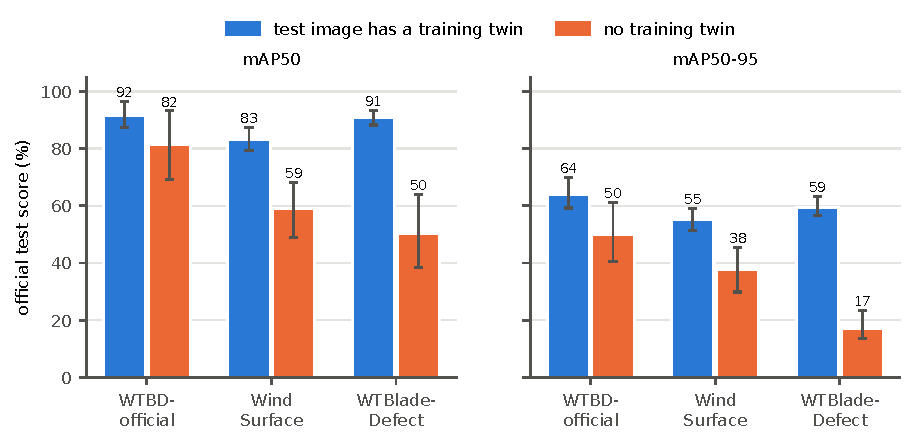
\includegraphics[width=\linewidth]{fig1_leak_subsets}
\caption{Official-protocol scores of the best RF-DETR-M run on leaked and no-twin test images, with image-bootstrap 95\% intervals.}
\label{fig:leak}
\end{figure}

WTBlade-Defect's official number is mostly its copies: 98.2 on copies of training frames and 50.4 with no same-scene training image. The independently built WTBlade-group benchmark agrees from a different direction. Its RF-DETR-M runs score 16.2--17.3 \mcoco (Table~\ref{tab:leakfree}) against 17.2 here, and their 38.5--41.6 \mfifty lies inside this small subset's interval of \ci{38.5}{64.0}. WTBD's no-twin subset is too small to read on its own: it holds a single box each of craze, thunderstrike and crack, and corrosion is the only class with a clear drop (\apfifty 97 to 54). The split comparison below is therefore the stronger evidence for WTBD.

\subsection{Same Detector, Only the Split Differs}
Table~\ref{tab:split-only} and Fig.~\ref{fig:inflation} compare models trained on the same 1{,}065 WTBD images, with the official split against the scene-grouped one.

\begin{table}[!t]
\centering
\caption{Same recipe, only the WTBD split differs: test \apfifty by class and overall \mfifty/\mcoco (O = official, G = group). BladeYOLO-v2 (BYv2) and YOLO12-L use Ultralytics \texttt{val}; RF-DETR-M uses the COCO-style evaluator, seed 0, 768\,px, 100 epochs on both splits. \best{Red bold}: best of the three models within each split.}
\label{tab:split-only}
\footnotesize
\setlength{\tabcolsep}{2.6pt}
\begin{tabular}{@{}l rr rr rr@{}}
\toprule
& \multicolumn{2}{c}{BYv2} & \multicolumn{2}{c}{YOLO12-L} & \multicolumn{2}{c}{RF-DETR-M} \\
\cmidrule(lr){2-3}\cmidrule(lr){4-5}\cmidrule(l){6-7}
Class & O & G & O & G & O & G \\
\midrule
crack & \best{99.1} & 38.1 & 85.4 & 38.4 & 95.3 & \best{61} \\
craze & 90.9 & 7.6 & 62.2 & 6.5 & \best{95.3} & \best{9} \\
hide\_craze & 80.0 & 56.9 & 63.9 & 52.6 & \best{80.3} & \best{71} \\
surface\_injure & 81.6 & 74.7 & 71.1 & 62.9 & \best{91.0} & \best{83} \\
thunderstrike & \best{99.5} & \best{98.0} & 93.8 & 41.8 & 94.3 & 64 \\
corrosion & 52.7 & 53.8 & 46.0 & \best{60.8} & \best{86.0} & 46 \\
\midrule
\mfifty & 84.0 & 54.8 & 70.4 & 43.8 & \best{90.4} & \best{55.3} \\
\mcoco & 49.3 & 24.5 & 38.8 & 20.6 & \best{61.2} & \best{33.2} \\
\bottomrule
\end{tabular}
\end{table}

\begin{figure}[!t]
\centering
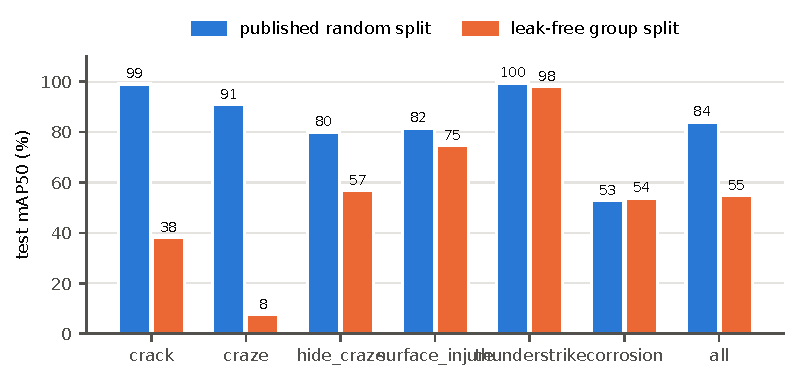
\includegraphics[width=0.95\linewidth]{fig3_wtbd_inflation}
\caption{Inflation per class on WTBD for BladeYOLO-v2 and YOLO12-L, with the same recipe on the official and the group split.}
\label{fig:inflation}
\end{figure}

The inflation does not depend on the model: $+29.2$ \mfifty for BladeYOLO-v2, $+26.6$ for YOLO12-L and $+35.1$ for RF-DETR-M, with \mcoco multiplied by 2.0, 1.9 and 1.8. On WTBlade the pair is 87.2/55.1 officially against 38.5/16.2 on WTBlade-group. That is not a pure split comparison, because WTBlade-group also keeps one frame per source and trains for 60 rather than 40 epochs.

\subsection{Tuning on the Official Splits Rewards Memorisation}
Between G25 and G26 we made one tuning step in the usual spirit. We moved to a cosine schedule (and, on two protocols, longer training) because the official numbers improved. Table~\ref{tab:tuning} decomposes what that step bought (post hoc).

\begin{table*}[!t]
\centering
\caption{What one tuning step bought, and what RF-DETR-FP changed. Paired image bootstrap, $\Delta$\mcoco in points on the same images. Interaction $=\Delta_{\mathrm{leaked}}-\Delta_{\mathrm{no\,twin}}$, with the subsets resampled independently.}
\label{tab:tuning}
\footnotesize
\begin{tabularx}{\textwidth}{@{}X l l l l@{}}
\toprule
Protocol (change) & $\Delta$ all & $\Delta$ leaked & $\Delta$ no twin & Interaction, $P(>0)$ \\
\midrule
\multicolumn{5}{@{}l}{\textit{G26 tuning step (post hoc)}} \\
WTBD-official (constant $\rightarrow$ cosine) & $+1.0$ \ci{-1.2}{+3.0} & $+1.8$ \ci{-0.1}{+4.0} & $-8.1$ \ci{-13.4}{+0.2} & $+9.9$ \ci{+1.1}{+15.8}, 0.993 \\
Wind Surface (60 ep constant $\rightarrow$ 100 ep cosine) & $+1.8$ \ci{+0.5}{+3.1} & $+2.3$ \ci{+0.9}{+3.8} & $-1.5$ \ci{-4.2}{+1.4} & $+3.8$ \ci{+0.7}{+7.0}, 0.988 \\
WTBlade-Defect (25 ep constant $\rightarrow$ 40 ep cosine) & $+2.6$ \ci{+1.1}{+3.9} & $+3.5$ \ci{+2.0}{+5.0}; copies $+5.4$ & $-4.0$ \ci{-7.2}{+0.1} & $+7.4$ \ci{+3.0}{+11.1}, 1.000 \\
\midrule
\multicolumn{5}{@{}l}{\textit{RF-DETR-FP $-$ its G26 twin (pre-registered benchmark entries)}} \\
\ours WTBD-official & $-1.2$ \ci{-3.3}{+1.0} & $-1.9$ \ci{-3.9}{+0.6} & $+2.6$ \ci{-2.1}{+7.2} & $-4.5$ \ci{-9.0}{+0.9}, 0.048 \\
\ours Wind Surface & $-1.5$ \ci{-2.9}{-0.3} & $-1.3$ \ci{-2.6}{+0.1} & $-2.3$ \ci{-6.7}{+2.0} & $+1.0$ \ci{-3.7}{+5.4}, 0.593 \\
\bottomrule
\end{tabularx}
\end{table*}

\begin{figure}[!t]
\centering
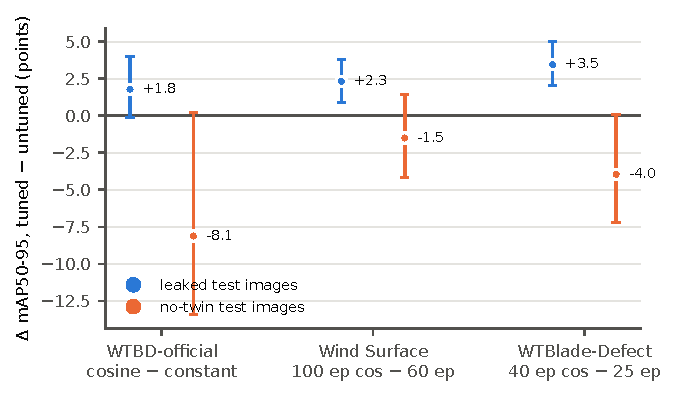
\includegraphics[width=\linewidth]{fig2_tuning_memorisation}
\caption{The G26 tuning step of Table~\ref{tab:tuning}: the gains sit on leaked images, and the same change lowers the no-twin score.}
\label{fig:tuning}
\end{figure}

On every protocol the gain of the tuning step sits on leaked images, and the same change lowers the score on images without a twin (Fig.~\ref{fig:tuning}). At \mfifty the change is $-0.2$ to $-0.8$ overall and $-5.0$ to $-6.0$ on no-twin images. The interaction excludes zero on all three protocols. This applies to our own G26 numbers, which stay in Table~\ref{tab:official} labelled as what they are. Two confounds remain: on Wind Surface and WTBlade-Defect the epoch count also changed (on WTBD only the schedule changed, with the same pattern), and this is one tuning step, not a study of tuning in general.

RF-DETR-FP moves in the opposite direction. On WTBD-official its change sits on the no-twin images ($+2.6$ \mcoco, $+9.2$ \mfifty), and the interaction is negative. By the rule fixed at pre-registration (no-twin $\Delta\geq0$), its official change is not memorisation. It is not an official \mcoco gain either, which falls on both protocols and significantly so on Wind Surface. A leaderboard reading would discard RF-DETR-FP; the leak-aware reading shows it is the only change we made whose official effect points towards unseen scenes.

A second reading comes from the leaderboard itself. RF-DETR-M leads BladeYOLO-v2 on WTBD-official by $+13.2$ \ci{+8.2}{+17.4} \mcoco on all images, but by only $+2.1$ \ci{-5.3}{+19.8} on the 36 no-twin images. That official lead is therefore not established on unseen images. RF-DETR-FP leads BladeYOLO-v2 by $+11.9$ \ci{+7.4}{+16.2} on all images and by $+4.7$ \ci{-4.2}{+23.4} on no-twin images.

\subsection{Consequence for Deployment: Leaked Calibration Breaks Recall Guarantees}
An inspection system should promise a bound on missed defects. Conformal risk control~\cite{crc} chooses a confidence threshold $\hat\lambda$ so that the expected share of missed defects is at most $\alpha$:
\begin{equation}
\hat\lambda=\sup\Big\{\lambda:\ \tfrac{n}{n+1}\hat{L}_n(\lambda)+\tfrac{1}{n+1}\leq\alpha\Big\},
\label{eq:crc}
\end{equation}
where $\hat{L}_n(\lambda)$ is the empirical miss rate on $n$ calibration units at threshold $\lambda$. A defect counts as flagged if at least 50\% of its box is covered by predictions above the threshold. We calibrate on seen or unseen scenes and always deploy on unseen scenes (Table~\ref{tab:conformal}, Fig.~\ref{fig:conformal}).

\begin{table}[!t]
\centering
\caption{Conformal recall guarantee, target $\leq$10\% missed (BladeYOLO-v2; 500 draws of 100 calibration images, or of scene groups as units).}
\label{tab:conformal}
\footnotesize
\begin{tabularx}{\linewidth}{@{}X X r r@{}}
\toprule
Calibrated on & Deployed on & Miss rate & Violating \\
\midrule
Seen scenes (group train), images & unseen scenes & \textbf{31.5\%} & 100\% \\
Seen scenes, scene units & unseen scenes & 28.8\% & 100\% \\
Unseen scenes (group val), images & unseen scenes & 6.3\% & 0\% \\
Unseen scenes, scene units & unseen scenes & 4.7\% & 1\% \\
Official val (leaky) & official test, with twin & 12.6\% & 91\% \\
Official val (leaky) & official test, no twin & \textbf{25.9\%} & 100\% \\
\bottomrule
\end{tabularx}
\end{table}

\begin{figure}[!t]
\centering
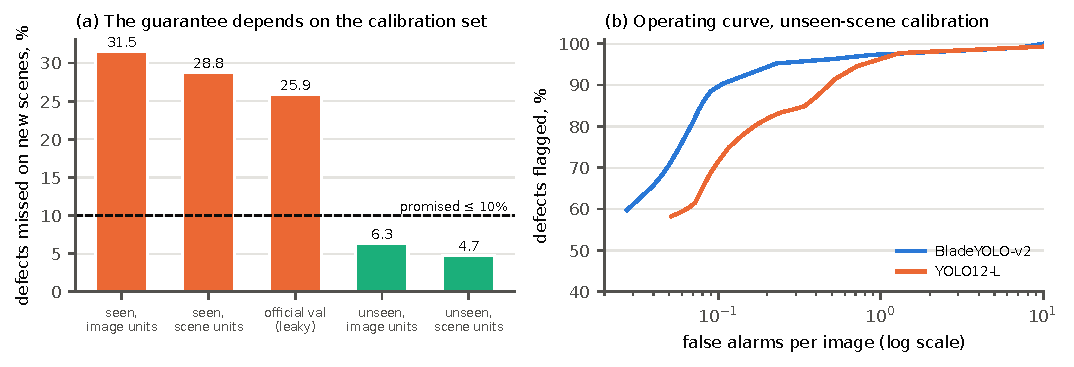
\includegraphics[width=\linewidth]{fig14_conformal}
\caption{(a) Realised miss rate on new scenes, by calibration set. (b) Operating curve with scene units, calibrated on unseen scenes. At 0.1 false alarms per image BladeYOLO-v2 flags about 90\% of defects on new scenes, YOLO12-L about 71\%. One test set of 58 scenes; the curve has no interval.}
\label{fig:conformal}
\end{figure}

Models are overconfident on what they memorised, so a threshold calibrated on seen scenes is too high for new data. Calibration data must therefore be split by scene, as test data must. The honest calibration is cheap: 0.2 instead of 0.1 false alarms per image. With only 60 calibration and 58 deployment scenes from one site, the validation and test groups are not perfectly exchangeable. YOLO12-L still misses 12.3\% with scene-unit calibration on unseen scenes, violating the bound in 71\% of draws.
